\documentclass[journal]{IEEEtran}
\usepackage{cite}
\usepackage{amsmath,amssymb}
\usepackage{graphicx}
\usepackage{booktabs}
\usepackage{tabularx}
\usepackage{array}
\usepackage{tikz}
\usepackage{xcolor}
\usepackage[hidelinks]{hyperref}
\usetikzlibrary{arrows.meta,positioning}

\graphicspath{{./Figures/}}

\begin{document}

\title{RetailPulse: A Databricks Lakehouse Framework for Grocery Order Analytics, Recommendation, and Validation}

\author{Harsh Vardhan, Anurag Nayak, Sameera Reddy, and Piyush Jain%
\thanks{Harsh Vardhan, Anurag Nayak, Sameera Reddy, and Piyush Jain are with the Department of Computer Science, Indian Institute of Information Technology, Nagpur, India, in the Branch of Computer Science and Engineering with Specialisation in Data Science and Analytics (e-mail: bt23csd041@iiitn.ac.in; bt23csd046@iiitn.ac.in; bt23csd057@iiitn.ac.in; bt23csd067@iiitn.ac.in).}}

\maketitle

\begin{abstract}
Retail analytics projects often emphasize models and dashboards while underreporting how data are curated, validated, and operationalized into reviewer-facing evidence. This paper presents RetailPulse, a Databricks lakehouse framework for grocery order analytics, recommendation, and validation built on the public Instacart order-history dataset. The system combines deterministic local sampling, explicit-schema ingestion, a bronze--silver--gold Delta pipeline, warehouse-style fact and dimension modeling, persisted OLAP summary tables, pairwise association-rule mining, KMeans-based customer segmentation, replay-style streaming validation, and a dashboard-oriented report layer. The framework is deliberately constrained by the realities of the source data and platform: the Instacart dataset contains no raw prices or absolute dates, and the validated execution target is Databricks Free Edition serverless. Results from the validated April 5, 2026 rebuild show populated bronze, silver, gold, and report tables; interpretable day-of-week demand summaries; actionable cross-sell rules and seed-product recommendations; three readable customer segments; and zero mismatches across 158 streamed order-slot validation groups. The paper also reports that physical-table optimization did not improve the benchmark queries on the current sample, and it explicitly demotes the supervised classifier and regression outputs to exploratory status because their methodology is not yet leakage-safe. RetailPulse demonstrates that a student-scale retail analytics system can still be engineered as a reproducible, evidence-backed lakehouse workflow rather than a collection of disconnected notebooks.
\end{abstract}

\begin{IEEEkeywords}
retail analytics, lakehouse, Databricks, market basket analysis, customer segmentation
\end{IEEEkeywords}

\section{Introduction}
Retail analytics is valuable only when its outputs can be reproduced, validated, and interpreted by someone other than the original notebook author. In practice, many small analytics projects fail in one of two ways: they remain exploratory notebook collections with weak data contracts, or they overstate predictive claims from loosely validated outputs. Modern lakehouse platforms promise a unified substrate for warehousing, analytics, and operational reporting \cite{armbrust2020deltalake,zaharia2021lakehouse}, but that promise still depends on disciplined pipeline design and explicit validation.

RetailPulse addresses this problem in the context of public grocery order history. The project is built on the Instacart order dataset \cite{instacart_dataset}, which is rich enough for basket analysis, reorder behavior, and customer segmentation, but not for price-based revenue analysis or calendar-based trend reporting. The validated execution target is Databricks Free Edition serverless \cite{databricks_free}, which supports Delta tables, SQL analytics, Structured Streaming, and AI/BI dashboards.

The paper is not positioned as an algorithmic novelty claim. Instead, it presents a framework contribution: a reproducible Databricks-first workflow that turns grocery order history into warehouse tables, recommendation evidence, descriptive analytics, customer segments, validation artifacts, and reviewer-facing outputs. The emphasis is on engineering quality and evidence packaging rather than on inventing a new recommender or clustering algorithm.

The main contributions of RetailPulse are as follows.
\begin{itemize}
    \item A deterministic sampling and ingestion workflow that converts public Instacart CSV files into a reproducible bronze--silver--gold Delta pipeline with explicit schemas and reusable report tables.
    \item An interpretable analytics layer that combines OLAP summaries, pairwise association-rule mining, and KMeans-based customer segmentation within the same warehouse contract.
    \item A validation-oriented execution layer that includes replay-style streaming checks, OLAP cross-checks, and benchmark reporting rather than relying on dashboard screenshots alone.
    \item A disciplined reporting strategy that separates release-safe descriptive evidence from exploratory supervised-model outputs whose methodology still requires redesign.
\end{itemize}

\section{Related Work}
\subsection{Retail Recommendation and Market Basket Analysis}
Retail recommendation has long relied on transactional co-occurrence patterns and collaborative filtering. Association-rule mining made basket analysis practical at scale by deriving frequent item relationships with interpretable support and confidence metrics \cite{agrawal1994association}, while later recommender work expanded toward item-based collaborative filtering \cite{sarwar2001itembased}. RetailPulse stays closer to the association-rule tradition because the project goal is auditable cross-sell evidence from order baskets rather than personalized ranking under dense feedback assumptions.

\subsection{Customer Segmentation and Clustering}
Customer segmentation is commonly used to summarize behavioral heterogeneity before any personalized intervention is attempted. KMeans remains a widely used baseline because it is simple, scalable, and easy to explain \cite{macqueen1967kmeans}. More recent work refines KMeans-based customer segmentation through feature engineering and optimization strategies \cite{li2021customersegmentation}. RetailPulse follows a descriptive segmentation lane: the goal is not to claim causal customer archetypes, but to create stable, warehouse-backed behavioral groups.

\subsection{Lakehouse and Streaming Analytics Systems}
The system dimension of retail analytics has also evolved. Delta Lake introduced ACID table storage and schema-aware management over cloud object stores \cite{armbrust2020deltalake}, while the lakehouse model argued for unifying warehousing and advanced analytics \cite{zaharia2021lakehouse}. Structured Streaming added a declarative model for integrating incremental processing with batch analytics \cite{armbrust2018structured}. RetailPulse builds on these ideas in a constrained educational setting using a Delta pipeline, Structured Streaming-compatible validation logic, and platform-native orchestration and dashboard layers. The addressed gap is integration: connecting descriptive analytics, recommendation evidence, validation, and reporting under explicit scope limits.

\section{Methodology and Proposed Work}
\subsection{Dataset and Analytical Scope}
RetailPulse uses the public Instacart order-history dataset \cite{instacart_dataset}. The dataset contains user-level grocery orders, order-item rows, products, aisles, and departments, which makes it suitable for basket analysis, reorder behavior, and user-level segmentation. However, it does not include raw prices, revenue, profit, or absolute calendar timestamps. The analytical scope of the framework is therefore intentionally limited to grocery order analytics rather than sales analytics. Operationally, the descriptive layer focuses on \texttt{order\_dow}, \texttt{order\_hour\_of\_day}, \texttt{days\_since\_prior\_order}, product affinities, and user-level shopping behavior.

\subsection{Deterministic Sampling and Ingestion}
The full Instacart dataset is sampled locally before upload to Databricks. The sampling script applies a deterministic rule based on user identity: by default, only users satisfying \texttt{user\_id \% 10 = 0} are retained, and the corresponding \texttt{order\_id} values are then used to filter the prior and train order-product files. This produces a stable 10\% subset without introducing randomness between runs. Lookup files for products, aisles, and departments are copied unchanged so the analytical vocabulary remains intact.

The sampled CSV files are uploaded into a Unity Catalog raw volume and ingested through explicit schemas. This step matters because it prevents hidden type drift and establishes a stable contract for downstream Delta tables. The ingestion and rebuild flow is packaged as a sequential reproducible job chain, which turns the notebook sequence into an execution unit rather than a manual classroom demo.

\subsection{Bronze--Silver--Gold Lakehouse Modeling}
After ingestion, RetailPulse organizes the data into a bronze--silver--gold pipeline. Bronze tables hold raw structured records with explicit schemas. Silver tables clean and enrich order and order-item data. Gold tables expose the reusable warehouse model required by later notebooks: \texttt{fact\_orders}, \texttt{fact\_order\_items}, supporting dimensions, and the \texttt{mart\_user\_features} table used for segmentation and exploratory predictive work. This design follows the practical lakehouse pattern of persisting reusable facts and dimensions rather than recomputing business logic directly inside dashboard queries \cite{armbrust2020deltalake,zaharia2021lakehouse}.

\begin{figure}[!t]
\centering
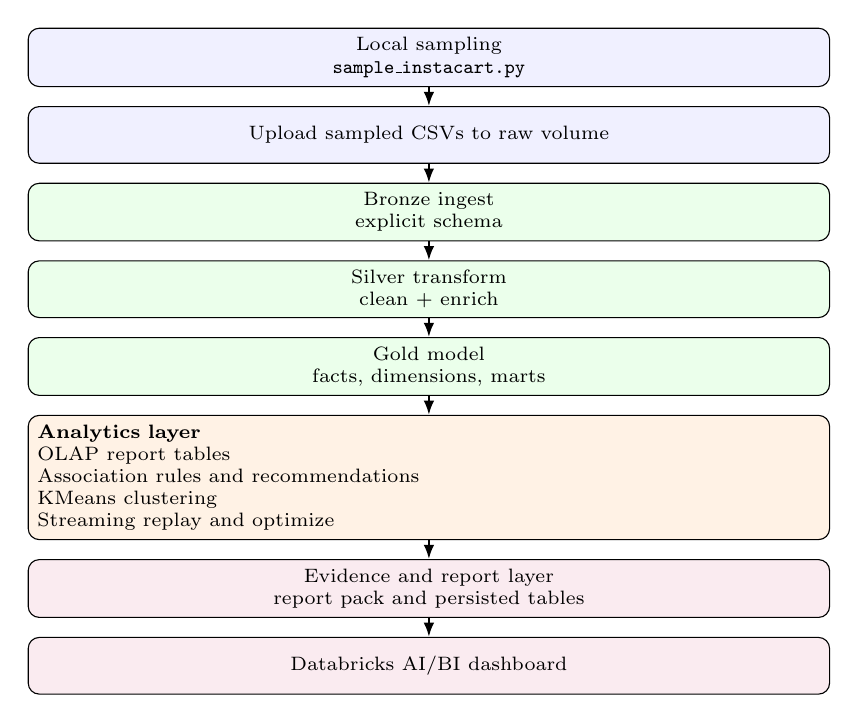
\begin{tikzpicture}[
    font=\scriptsize,
    node distance=0.24cm,
    box/.style={draw, rounded corners, align=center, text width=0.82\columnwidth, minimum height=0.72cm, fill=blue!6},
    stage/.style={draw, rounded corners, align=center, text width=0.82\columnwidth, minimum height=0.72cm, fill=green!8},
    analytic/.style={draw, rounded corners, align=left, text width=0.82\columnwidth, minimum height=1.35cm, fill=orange!10},
    output/.style={draw, rounded corners, align=center, text width=0.82\columnwidth, minimum height=0.72cm, fill=purple!8},
    arr/.style={-{Latex[length=1.8mm]}, thick}
]
\node[box] (sample) {Local sampling\\\texttt{sample\_instacart.py}};
\node[box, below=of sample] (upload) {Upload sampled CSVs to raw volume};
\node[stage, below=of upload] (bronze) {Bronze ingest\\explicit schema};
\node[stage, below=of bronze] (silver) {Silver transform\\clean + enrich};
\node[stage, below=of silver] (gold) {Gold model\\facts, dimensions, marts};
\node[analytic, below=of gold] (analytics) {\textbf{Analytics layer}\\OLAP report tables\\Association rules and recommendations\\KMeans clustering\\Streaming replay and optimize};
\node[output, below=of analytics] (report) {Evidence and report layer\\report pack and persisted tables};
\node[output, below=of report] (dashboard) {Databricks AI/BI dashboard};

\draw[arr] (sample) -- (upload);
\draw[arr] (upload) -- (bronze);
\draw[arr] (bronze) -- (silver);
\draw[arr] (silver) -- (gold);
\draw[arr] (gold) -- (analytics);
\draw[arr] (analytics) -- (report);
\draw[arr] (report) -- (dashboard);
\end{tikzpicture}
\caption{RetailPulse end-to-end workflow. Deterministic local sampling feeds a Databricks bronze--silver--gold pipeline, after which analytics, evidence tables, and dashboard outputs are generated from persisted Delta tables.}
\label{fig:end_to_end}
\end{figure}

\subsection{OLAP and Report Table Generation}
The descriptive analytics layer is materialized rather than left implicit in notebook outputs. RetailPulse runs a set of OLAP-oriented queries: a cube over department and day-of-week demand, a rollup over day-of-week and hour-of-day order behavior, and a basket-analysis aggregation by daypart and department. The resulting tables are persisted as report artifacts so the dashboard and the report pack can read them without recomputing logic.

The same notebook also produces a validation table by comparing base-grain cube totals against a direct aggregation over the fact table. This validation step is important because it turns descriptive analytics into a checkable contract instead of a purely visual layer.

\subsection{Analytical Formulation}
The implementation above is encoded with explicit mathematical contracts so each release-safe claim can be traced to a persisted table. Let \(U\) be the set of distinct users in the raw orders file. Deterministic sampling retains
\begin{equation}
S = \{u \in U \mid u \bmod 10 = 0\}.
\end{equation}
For each sampled user, all related orders and order-items are included, producing a stable \(10\%\) user slice across reruns.

For pairwise association rules \(X \rightarrow Y\), with \(N\) baskets and indicator \(\mathbf{1}[\cdot]\), the mined metrics are
\begin{equation}
\mathrm{supp}(X \rightarrow Y) = \frac{1}{N}\sum_{i=1}^{N}\mathbf{1}[X \cup Y \subseteq B_i],
\end{equation}
\begin{equation}
\mathrm{conf}(X \rightarrow Y) = \frac{\mathrm{supp}(X \rightarrow Y)}{\mathrm{supp}(X)},
\end{equation}
\begin{equation}
\mathrm{lift}(X \rightarrow Y) = \frac{\mathrm{conf}(X \rightarrow Y)}{\mathrm{supp}(Y)}.
\end{equation}

For clustering, each user feature vector \(\mathbf{x}_u\) is standardized component-wise as
\begin{equation}
\mathbf{z}_u = \left(\frac{x_{u,1}-\mu_1}{\sigma_1},\ldots,\frac{x_{u,d}-\mu_d}{\sigma_d}\right),
\end{equation}
and KMeans minimizes
\begin{equation}
J_k = \sum_{j=1}^{k}\sum_{\mathbf{z}_u \in C_j}\lVert\mathbf{z}_u-\boldsymbol{\mu}_j\rVert_2^2,
\end{equation}
with model selection over \(k \in \{3,4,5\}\) by maximizing average silhouette score \cite{rouseeuw1987silhouettes}:
\begin{equation}
k^* = \arg\max_{k \in \{3,4,5\}}\frac{1}{|S_k|}\sum_{u \in S_k}s(u).
\end{equation}

For replay-stream validation, let \(G\) denote the set of \((\texttt{order\_dow},\texttt{order\_hour\_of\_day})\) groups. Exact agreement for group \(g \in G\) is
\begin{equation}
m(g)=\mathbf{1}\!\left[(c_g^\mathrm{stream}, b_g^\mathrm{stream}, r_g^\mathrm{stream})=(c_g^\mathrm{batch}, b_g^\mathrm{batch}, r_g^\mathrm{batch})\right],
\end{equation}
and mismatch count is
\begin{equation}
M = \sum_{g \in G} (1-m(g)).
\end{equation}
The release criterion for streaming correctness is \(M=0\).

\subsection{Pairwise Association-Rule Mining}
Recommendation evidence is derived from \texttt{fact\_order\_items}. For each order, RetailPulse collects the distinct product identifiers, enumerates pairwise item co-occurrences within the same basket, and computes support, confidence, and lift in the classical association-rule sense \cite{agrawal1994association}. The rules are filtered using configurable thresholds, with the validated baseline using minimum support \texttt{0.005} and minimum confidence \texttt{0.2}. The resulting \texttt{mart\_association\_rules} table is the reusable recommendation surface for both top-rule inspection and seed-product recommendation examples.

This implementation choice is deliberate. Full FP-growth would be a natural extension, but the current project favors a serverless-safe, easy-to-audit pairwise rule pipeline over a more ambitious mining stack that is harder to operationalize on the constrained target platform.

\subsection{KMeans-Based Customer Segmentation}
Customer segmentation is built on the warehouse-level \texttt{mart\_user\_features} table. The clustering notebook assembles and standardizes seven features: total orders, average basket size, average days since prior order, average reordered-item rate, average distinct department count, average order hour of day, and active days. KMeans is then evaluated for \(k \in \{3,4,5\}\), and silhouette score is used to select the best value of \(k\) \cite{macqueen1967kmeans}. The winning assignments are written back to the user mart, and cluster-level profile summaries are materialized in a dedicated report table.

The purpose of this step is interpretability. Clusters are treated as descriptive audience groups that help organize downstream recommendation and dashboard discussion, not as stable latent customer identities.

\subsection{Replay-Style Streaming Validation}
RetailPulse includes a replay-style streaming notebook because the project aims to validate incremental processing behavior, not just warehouse snapshots. A deterministic held-out slice of \texttt{fact\_orders} is partitioned into four CSV batches and written into a replay volume. The replay is then consumed through a Structured Streaming pipeline that groups orders by day of week and hour of day, using \texttt{Trigger.AvailableNow} to remain compatible with the Databricks Free Edition serverless environment \cite{armbrust2018structured,databricks_free}.

The streamed aggregates are compared against a batch recomputation at the same order-slot grain. The validation table records whether order counts, average basket size, and reordered-item totals match exactly. Any mismatch is treated as a correctness failure rather than a tolerable approximation.

\subsection{Exploratory Predictive Lane}
The framework also includes a secondary predictive lane. One notebook trains a decision-tree classifier to predict whether a user belongs to the top quartile of total orders; another trains a linear regression model to estimate basket size from order context and user-level history. These outputs are persisted because they are useful for demo discussion and feature inspection, but they are not part of the framework's release-safe proof. As discussed later, the current feature design still contains leakage risk and therefore does not justify production-grade predictive claims.

\section{Results and Analysis}
\subsection{Validated Execution and Table Population}
The manuscript evaluates the validated April 5, 2026 release state of RetailPulse. The authoritative rebuild facts are summarized in Table~\ref{tab:run_facts}. Table~\ref{tab:validated_counts} shows that the bronze, silver, gold, and report layers were populated end to end. The counts also confirm that recommendation, clustering, validation, and optimization outputs were materialized rather than left as transient notebook displays.

\begin{table}[!t]
\caption{Validated RetailPulse execution facts.}
\label{tab:run_facts}
\centering
\footnotesize
\begin{tabular}{p{2.9cm} p{4.7cm}}
\toprule
\textbf{Item} & \textbf{Value} \\
\midrule
Workspace target & Databricks Free Edition serverless \\
Bundle job name & \texttt{retailpulse\_full\_rebuild} \\
Job id & \texttt{61936309152043} \\
Successful run id & \texttt{631388168060027} \\
Dashboard & \texttt{RetailPulse Demo Dashboard} \\
Dashboard revision & \texttt{2026-04-05T08:40:02.619Z} \\
\bottomrule
\end{tabular}
\end{table}

\begin{table}[!t]
\caption{Validated table population counts.}
\label{tab:validated_counts}
\centering
\footnotesize
\begin{tabular}{p{4.8cm} r}
\toprule
\textbf{Table} & \textbf{Rows} \\
\midrule
\texttt{bronze\_orders} & 341,974 \\
\texttt{silver\_order\_items} & 3,405,038 \\
\texttt{fact\_order\_items} & 3,405,038 \\
\texttt{fact\_orders} & 334,438 \\
\texttt{mart\_association\_rules} & 49 \\
\texttt{report\_cluster\_profiles} & 3 \\
\texttt{report\_cluster\_k\_scores} & 3 \\
\texttt{report\_stream\_validation} & 158 \\
\texttt{report\_optimize\_summary} & 2 \\
\bottomrule
\end{tabular}
\end{table}

\subsection{Order Behavior and OLAP Findings}
The descriptive layer converts the gold facts into reusable analytical summaries. Figure~\ref{fig:olap_outputs} is the primary full-width OLAP view showing department demand and hourly timing behavior from persisted report tables as rendered by dashboard widgets. Figure~\ref{fig:orders_by_day} complements this with the day-of-week rollup that combines order counts with average basket size.

The same OLAP notebook also produces product-concentration evidence; Figure~\ref{fig:top_products} surfaces the top-product widget backed by the same persisted analytical layer. Because the source dataset does not contain absolute dates, findings are intentionally phrased in terms of relative day and hour behavior rather than calendar seasonality.

\begin{figure*}[!t]
\centering
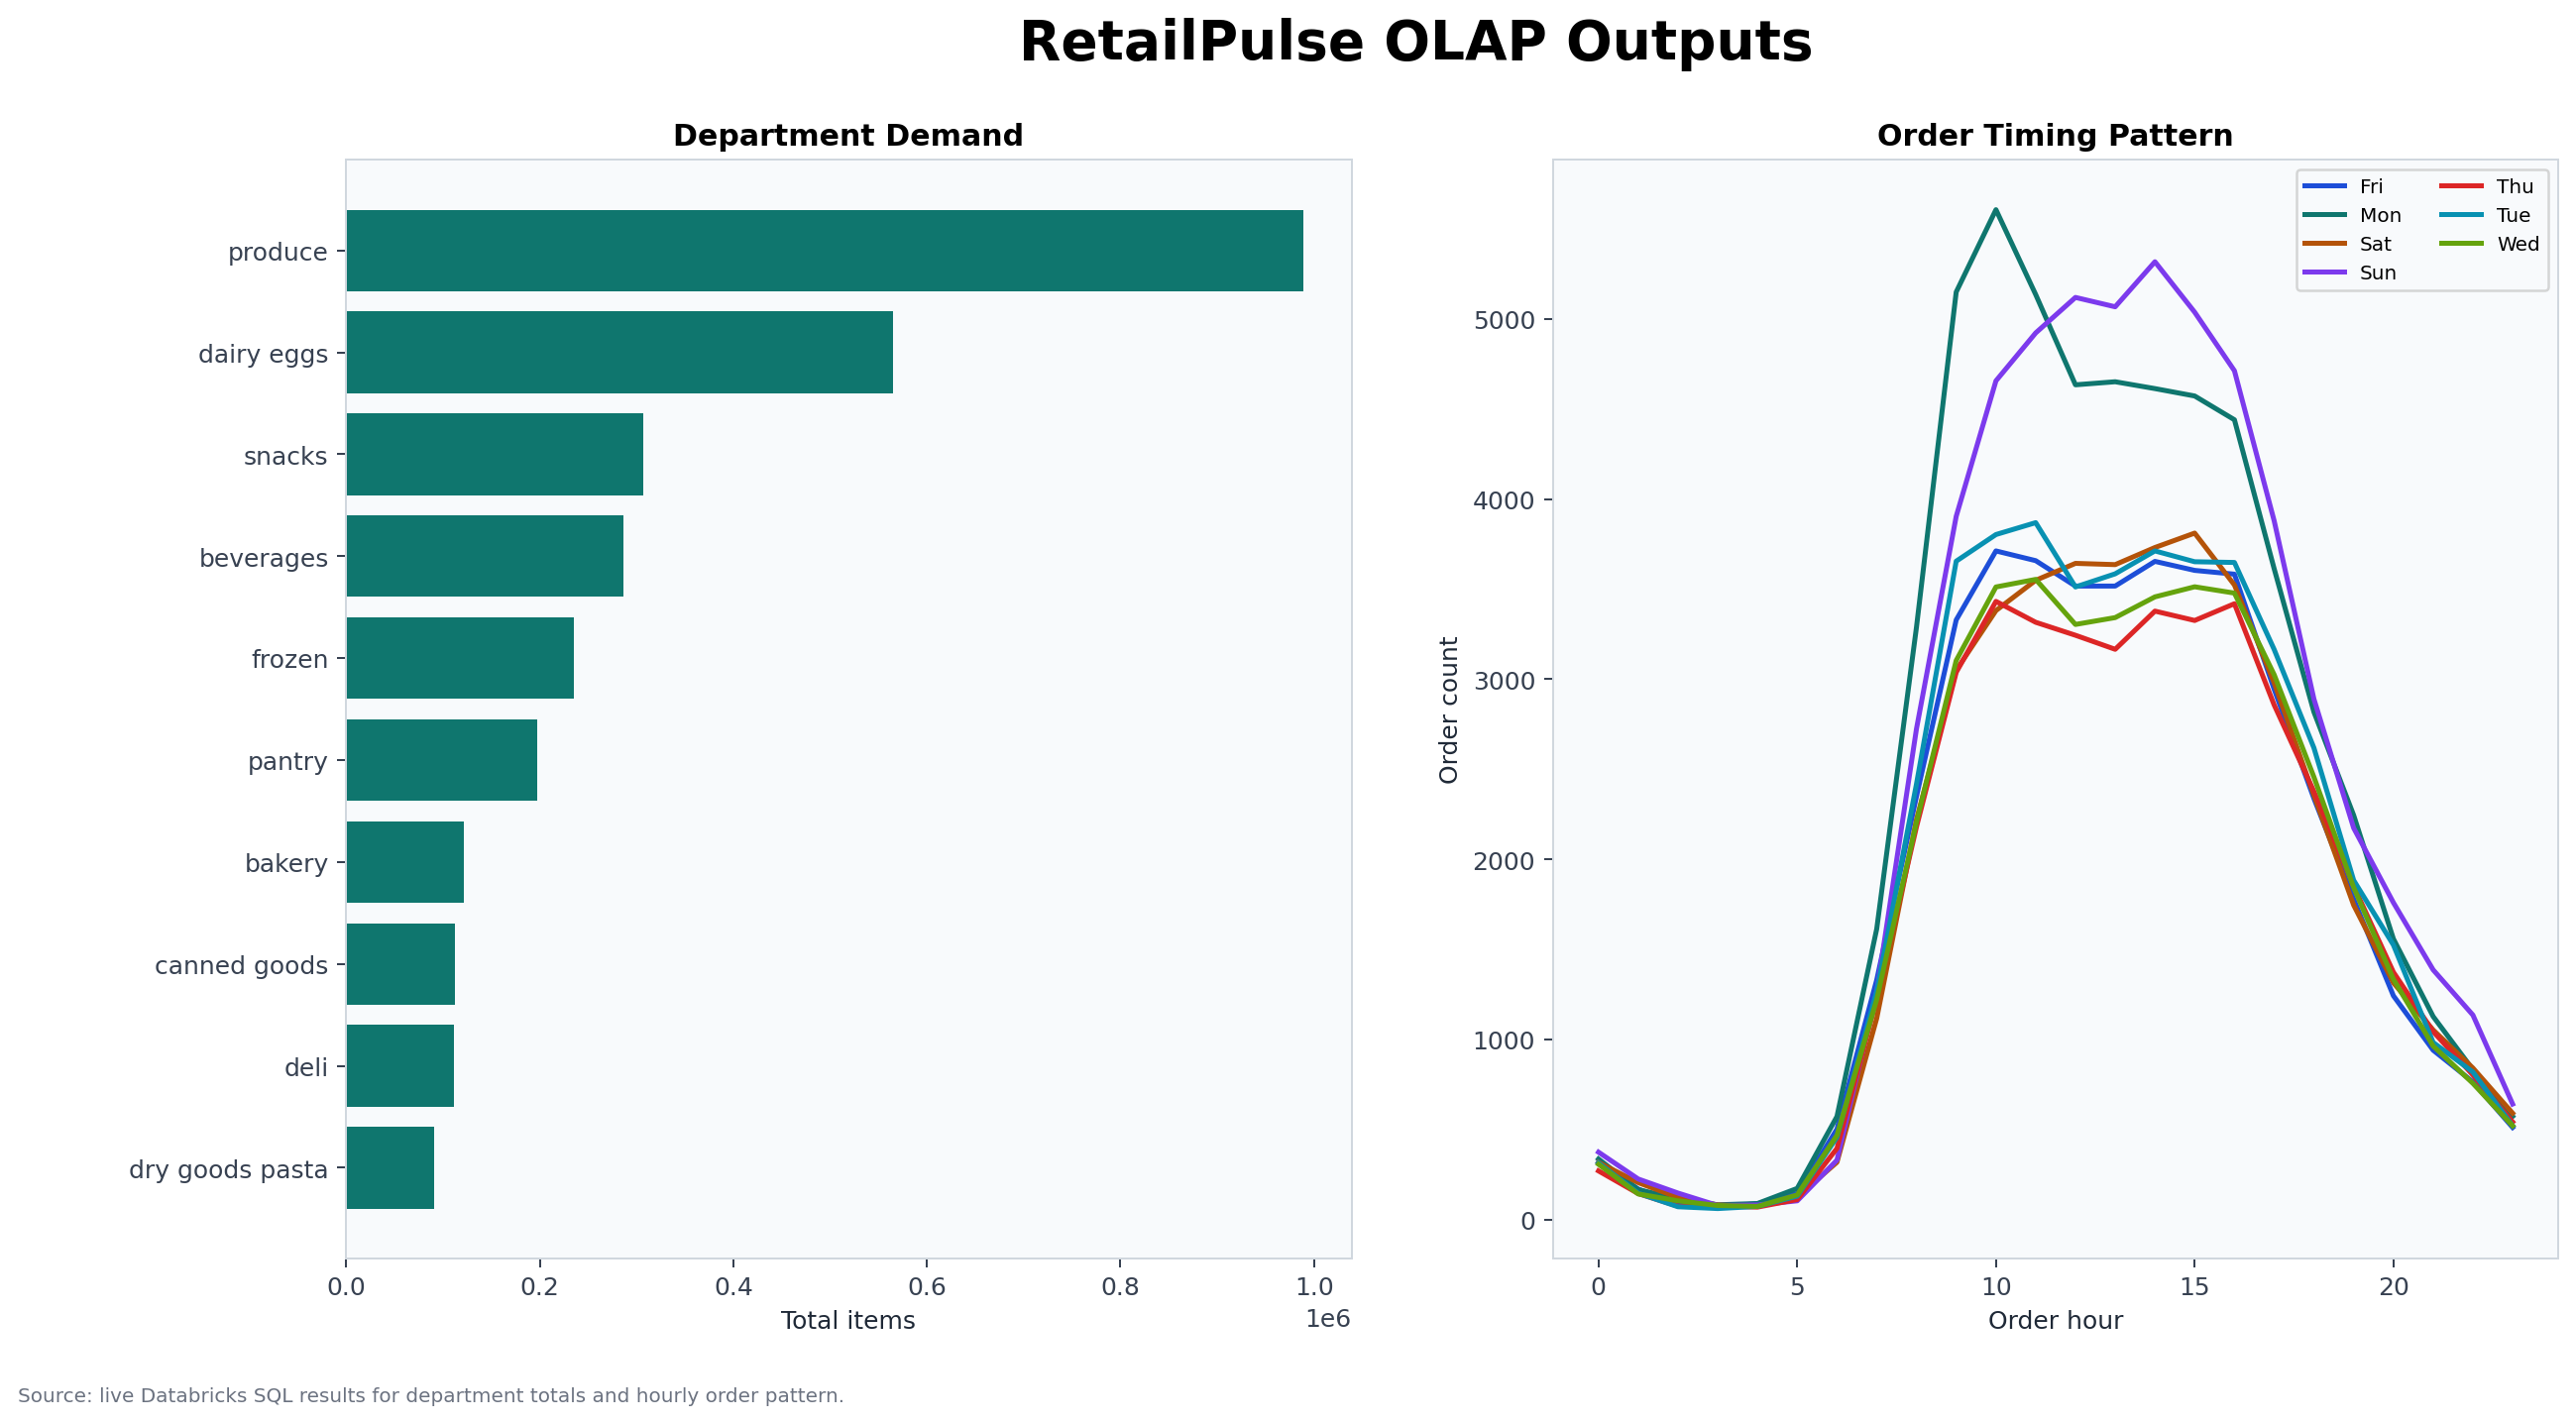
\includegraphics[width=\textwidth]{03_olap_outputs.png}
\caption{Full-width OLAP evidence from persisted report tables, surfaced in dashboard widgets for department-demand and hourly-order behavior.}
\label{fig:olap_outputs}
\end{figure*}

\begin{figure}[!t]
\centering
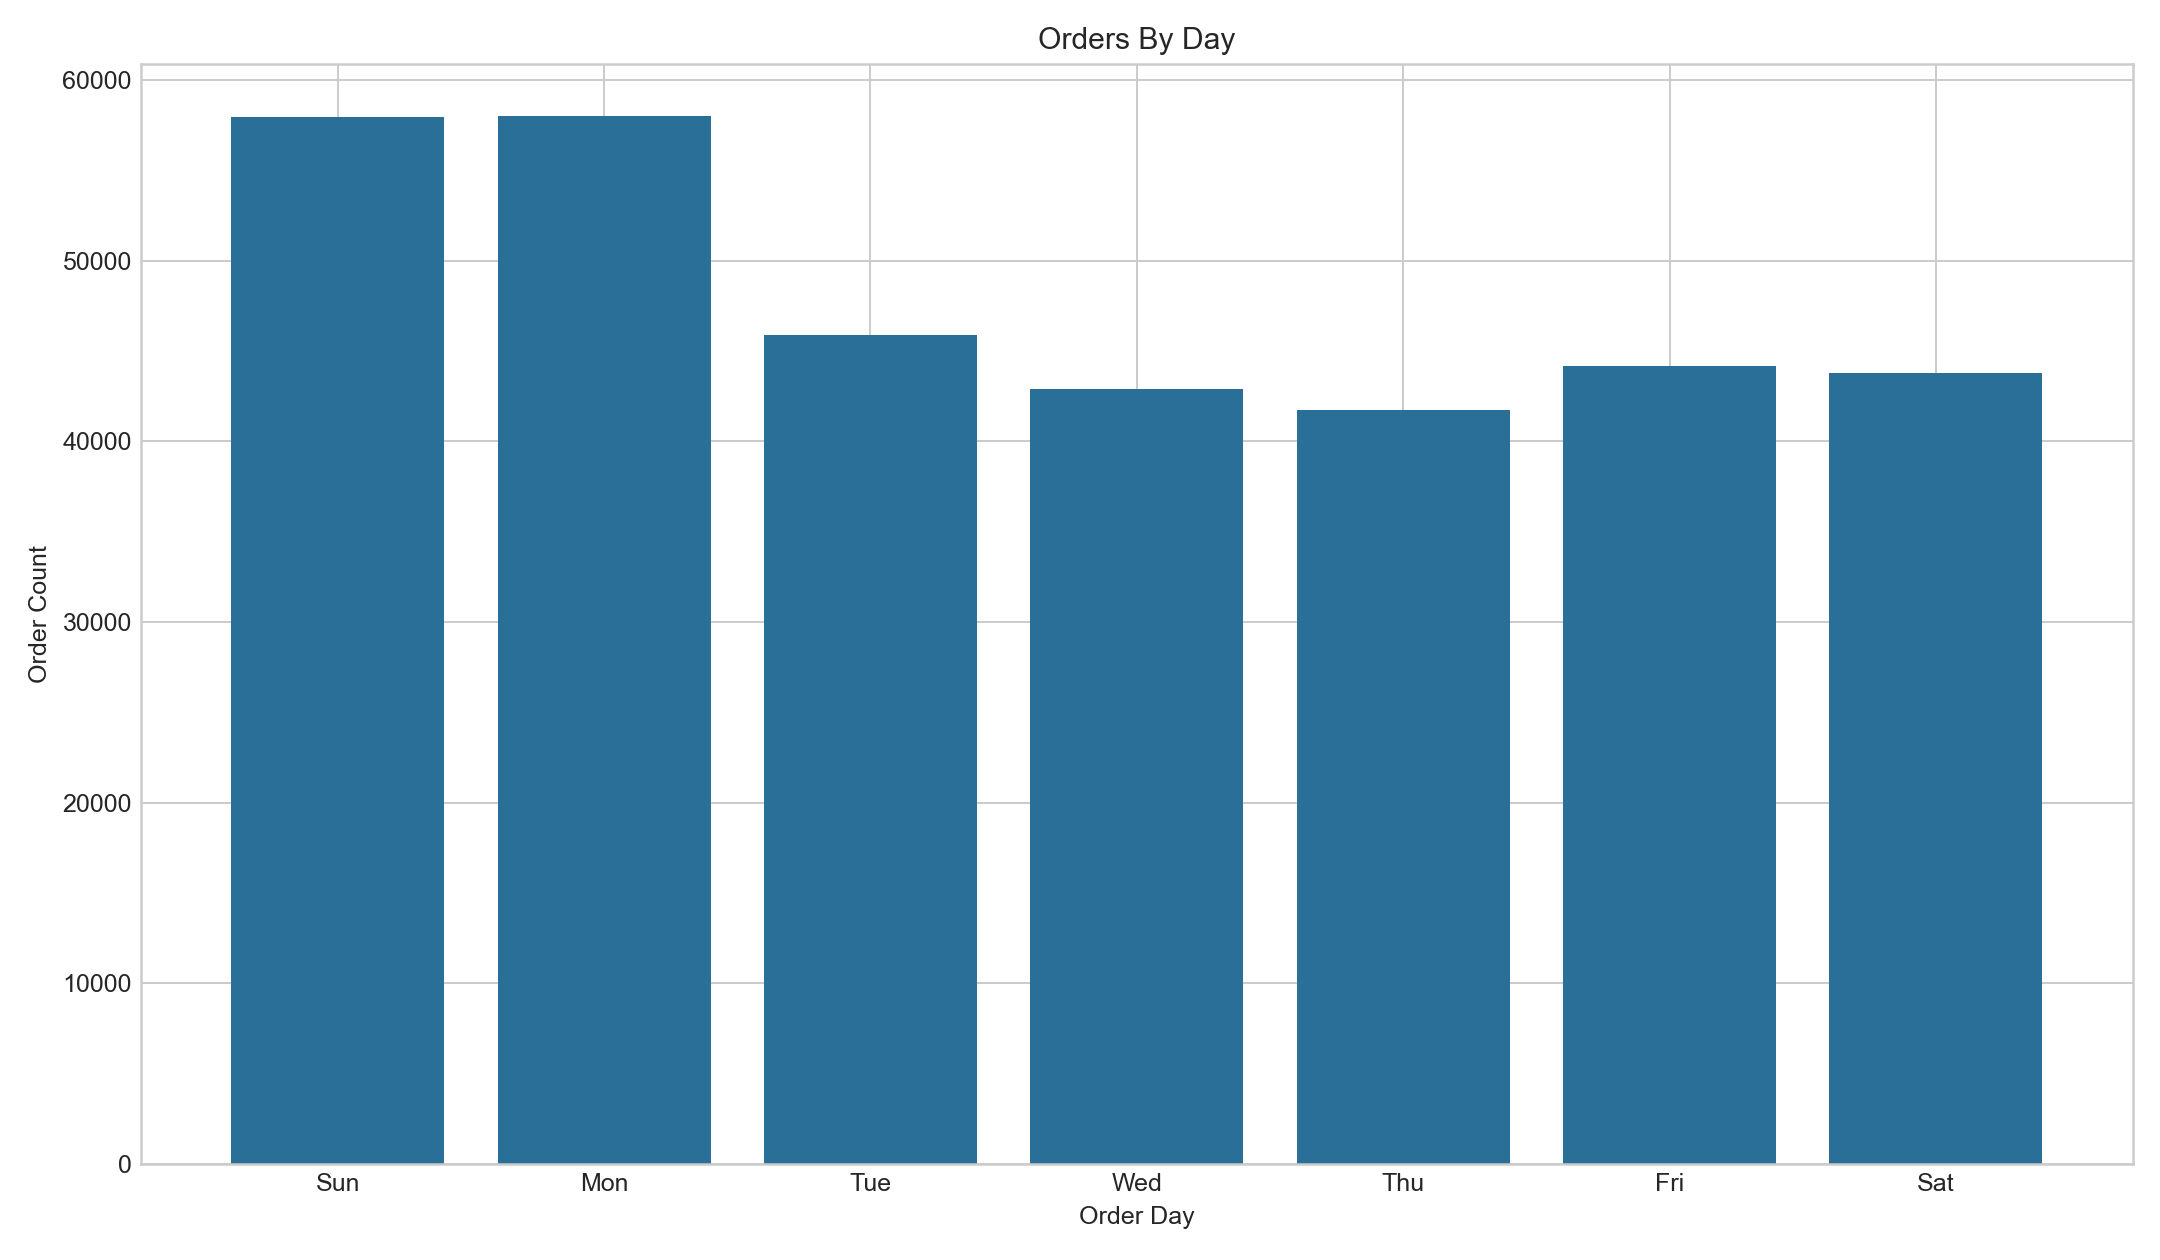
\includegraphics[width=\columnwidth]{10_orders_by_day.png}
\caption{Order-behavior evidence from the persisted day-of-week rollup table used by the dashboard query surface. The chart summarizes order-count and average-basket behavior by \texttt{order\_dow}.}
\label{fig:orders_by_day}
\end{figure}

\begin{figure}[!t]
\centering
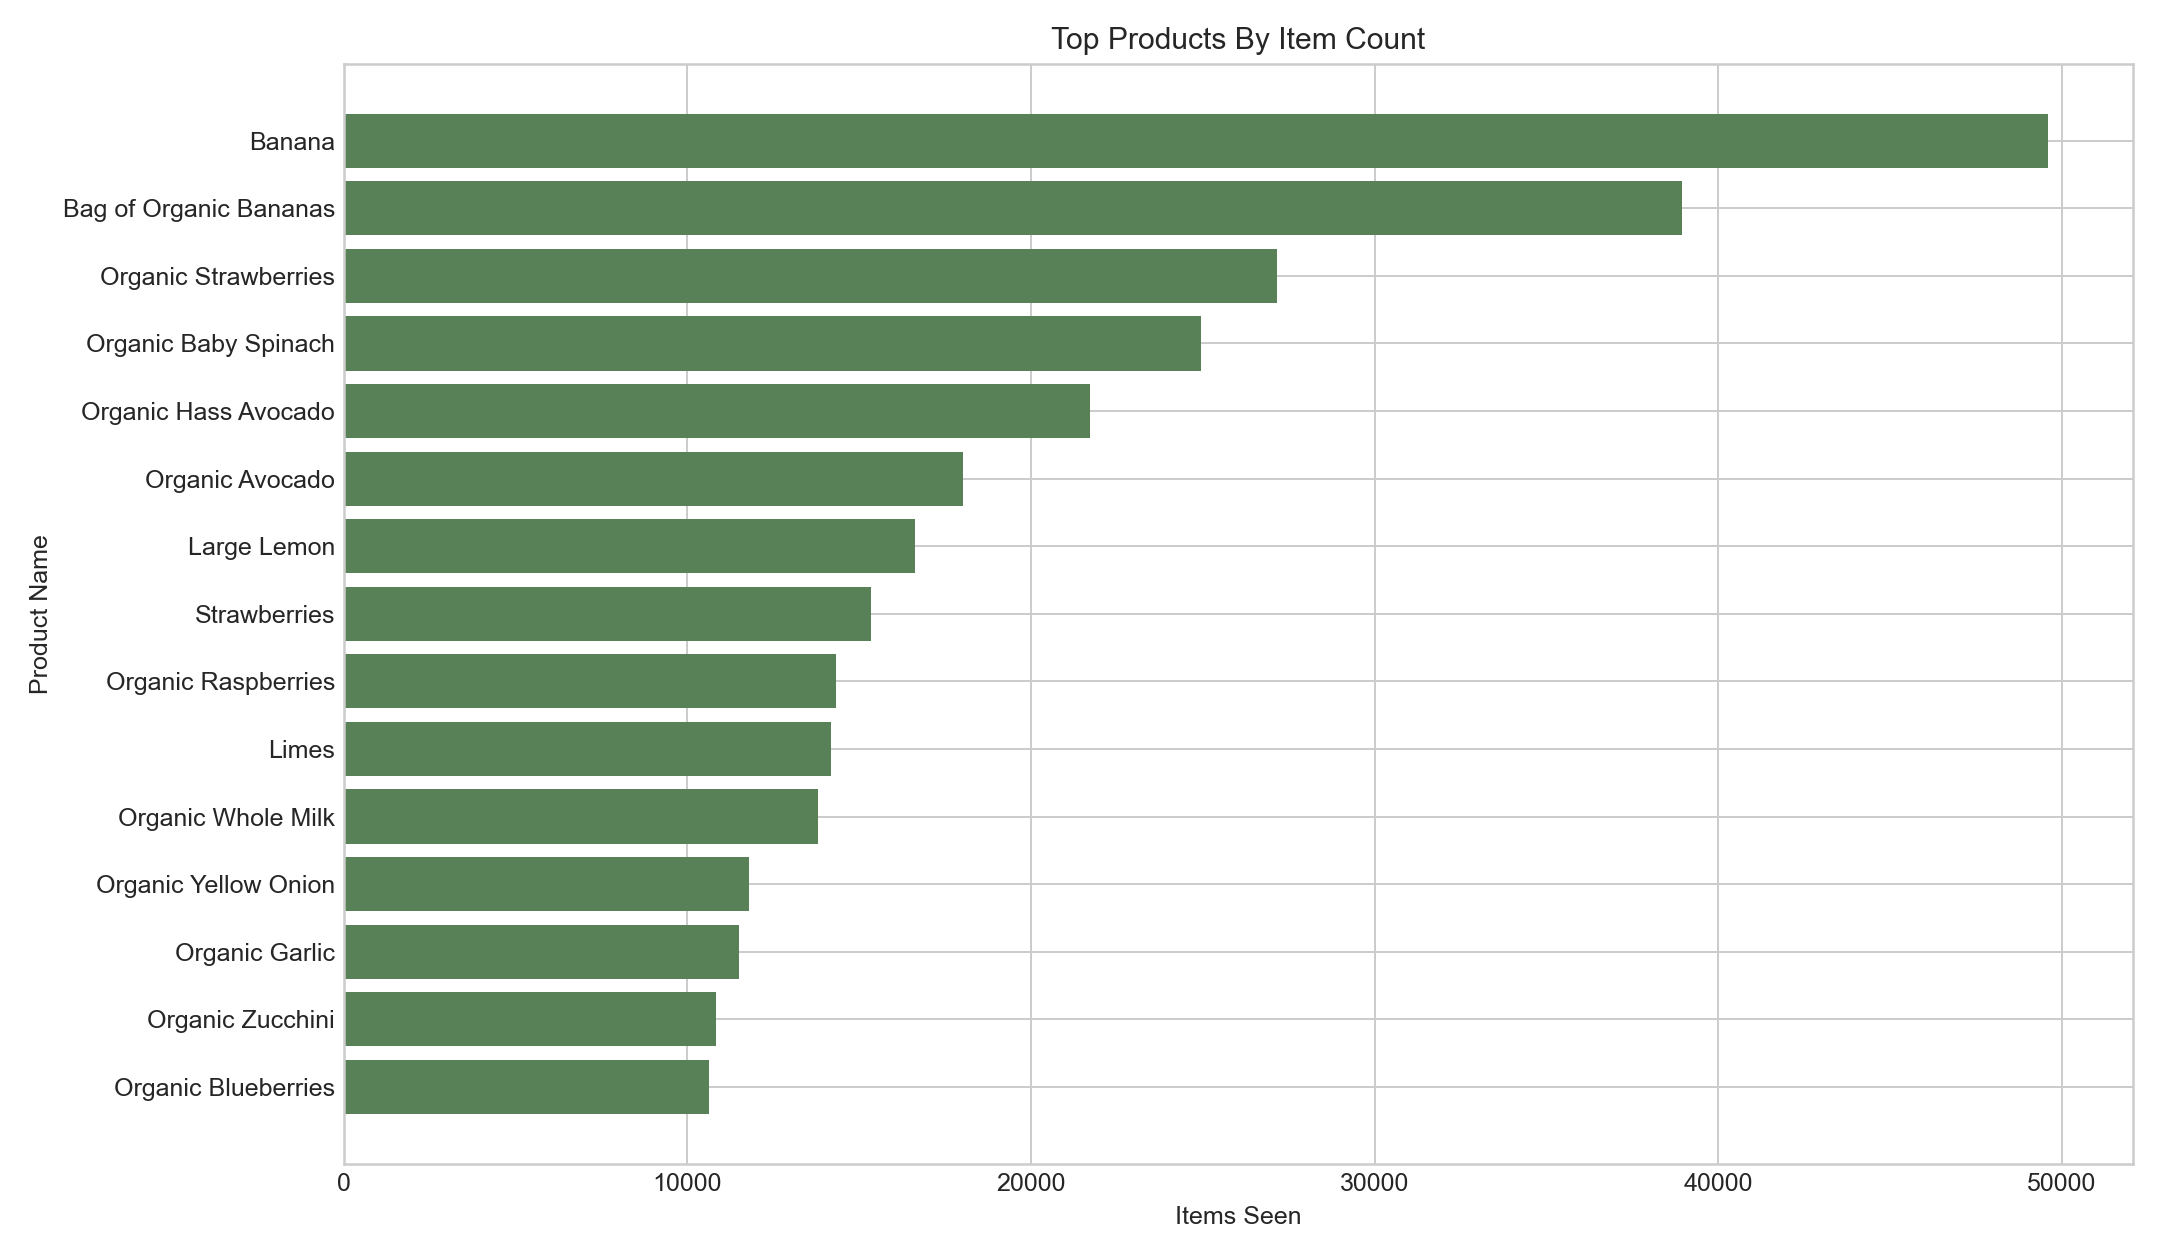
\includegraphics[width=\columnwidth]{11_top_products.png}
\caption{Product-concentration evidence from the persisted top-products dashboard widget, showing dominant products in the validated sample.}
\label{fig:top_products}
\end{figure}

\subsection{Recommendation and Segmentation Findings}
The recommendation path yields interpretable product affinities. Table~\ref{tab:top_rule} shows a representative rule from the validated rule mart: \emph{Organic Garlic} implies \emph{Organic Yellow Onion} with support \(0.0073\), confidence \(0.2018\), and lift \(5.4620\). These values matter jointly: support shows recurrence, confidence shows directional strength, and lift indicates that the pair co-occurs far more often than an independence baseline would suggest.

The same persisted rule mart supports seed-product recommendation output. Table~\ref{tab:seed_recommendation} shows the validated example for \emph{Organic Raspberries}, which returns \emph{Bag of Organic Bananas} and \emph{Organic Strawberries}. This is a useful demonstration of how a reusable rule table can be turned into an actionable next-best-product view without introducing a separate recommender stack.

The segmentation lane also produced readable customer groups. Table~\ref{tab:cluster_profiles} shows that cluster \(0\) behaves like frequent loyal shoppers, cluster \(1\) behaves like light occasional shoppers, and cluster \(2\) emphasizes large-basket stock-up behavior. Figure~\ref{fig:k_selection} exposes the model-selection evidence across the tested \(k\) values, which is necessary if the segmentation result is to be interpreted as a justified descriptive summary rather than an arbitrary clustering output.

\begin{table}[!t]
\caption{Representative association rule from the validated recommendation mart.}
\label{tab:top_rule}
\centering
\footnotesize
\begin{tabular}{p{1.7cm} p{1.8cm} r r r}
\toprule
\textbf{Antecedent} & \textbf{Consequent} & \textbf{Support} & \textbf{Confidence} & \textbf{Lift} \\
\midrule
Organic Garlic & Organic Yellow Onion & 0.0073 & 0.2018 & 5.4620 \\
\bottomrule
\end{tabular}
\end{table}

\begin{table}[!t]
\caption{Validated seed-product recommendation example.}
\label{tab:seed_recommendation}
\centering
\footnotesize
\begin{tabular}{p{2.5cm} p{4.0cm}}
\toprule
\textbf{Seed product} & \textbf{Recommended products} \\
\midrule
Organic Raspberries & Bag of Organic Bananas; Organic Strawberries \\
\bottomrule
\end{tabular}
\end{table}

\begin{table}[!t]
\caption{Validated cluster-profile summary.}
\label{tab:cluster_profiles}
\centering
\footnotesize
\begin{tabular}{p{0.4cm} p{2.2cm} p{2.0cm} r}
\toprule
\textbf{ID} & \textbf{Profile} & \textbf{Metric} & \textbf{Value} \\
\midrule
0 & Frequent loyal shoppers & Avg total orders & 33.28 \\
0 & Frequent loyal shoppers & Reorder rate & 0.6521 \\
1 & Light occasional shoppers & Avg total orders & 7.54 \\
1 & Light occasional shoppers & Avg basket size & 6.63 \\
2 & Large-basket stock-up shoppers & Avg basket size & 17.12 \\
\bottomrule
\end{tabular}
\end{table}

\begin{figure}[!t]
\centering
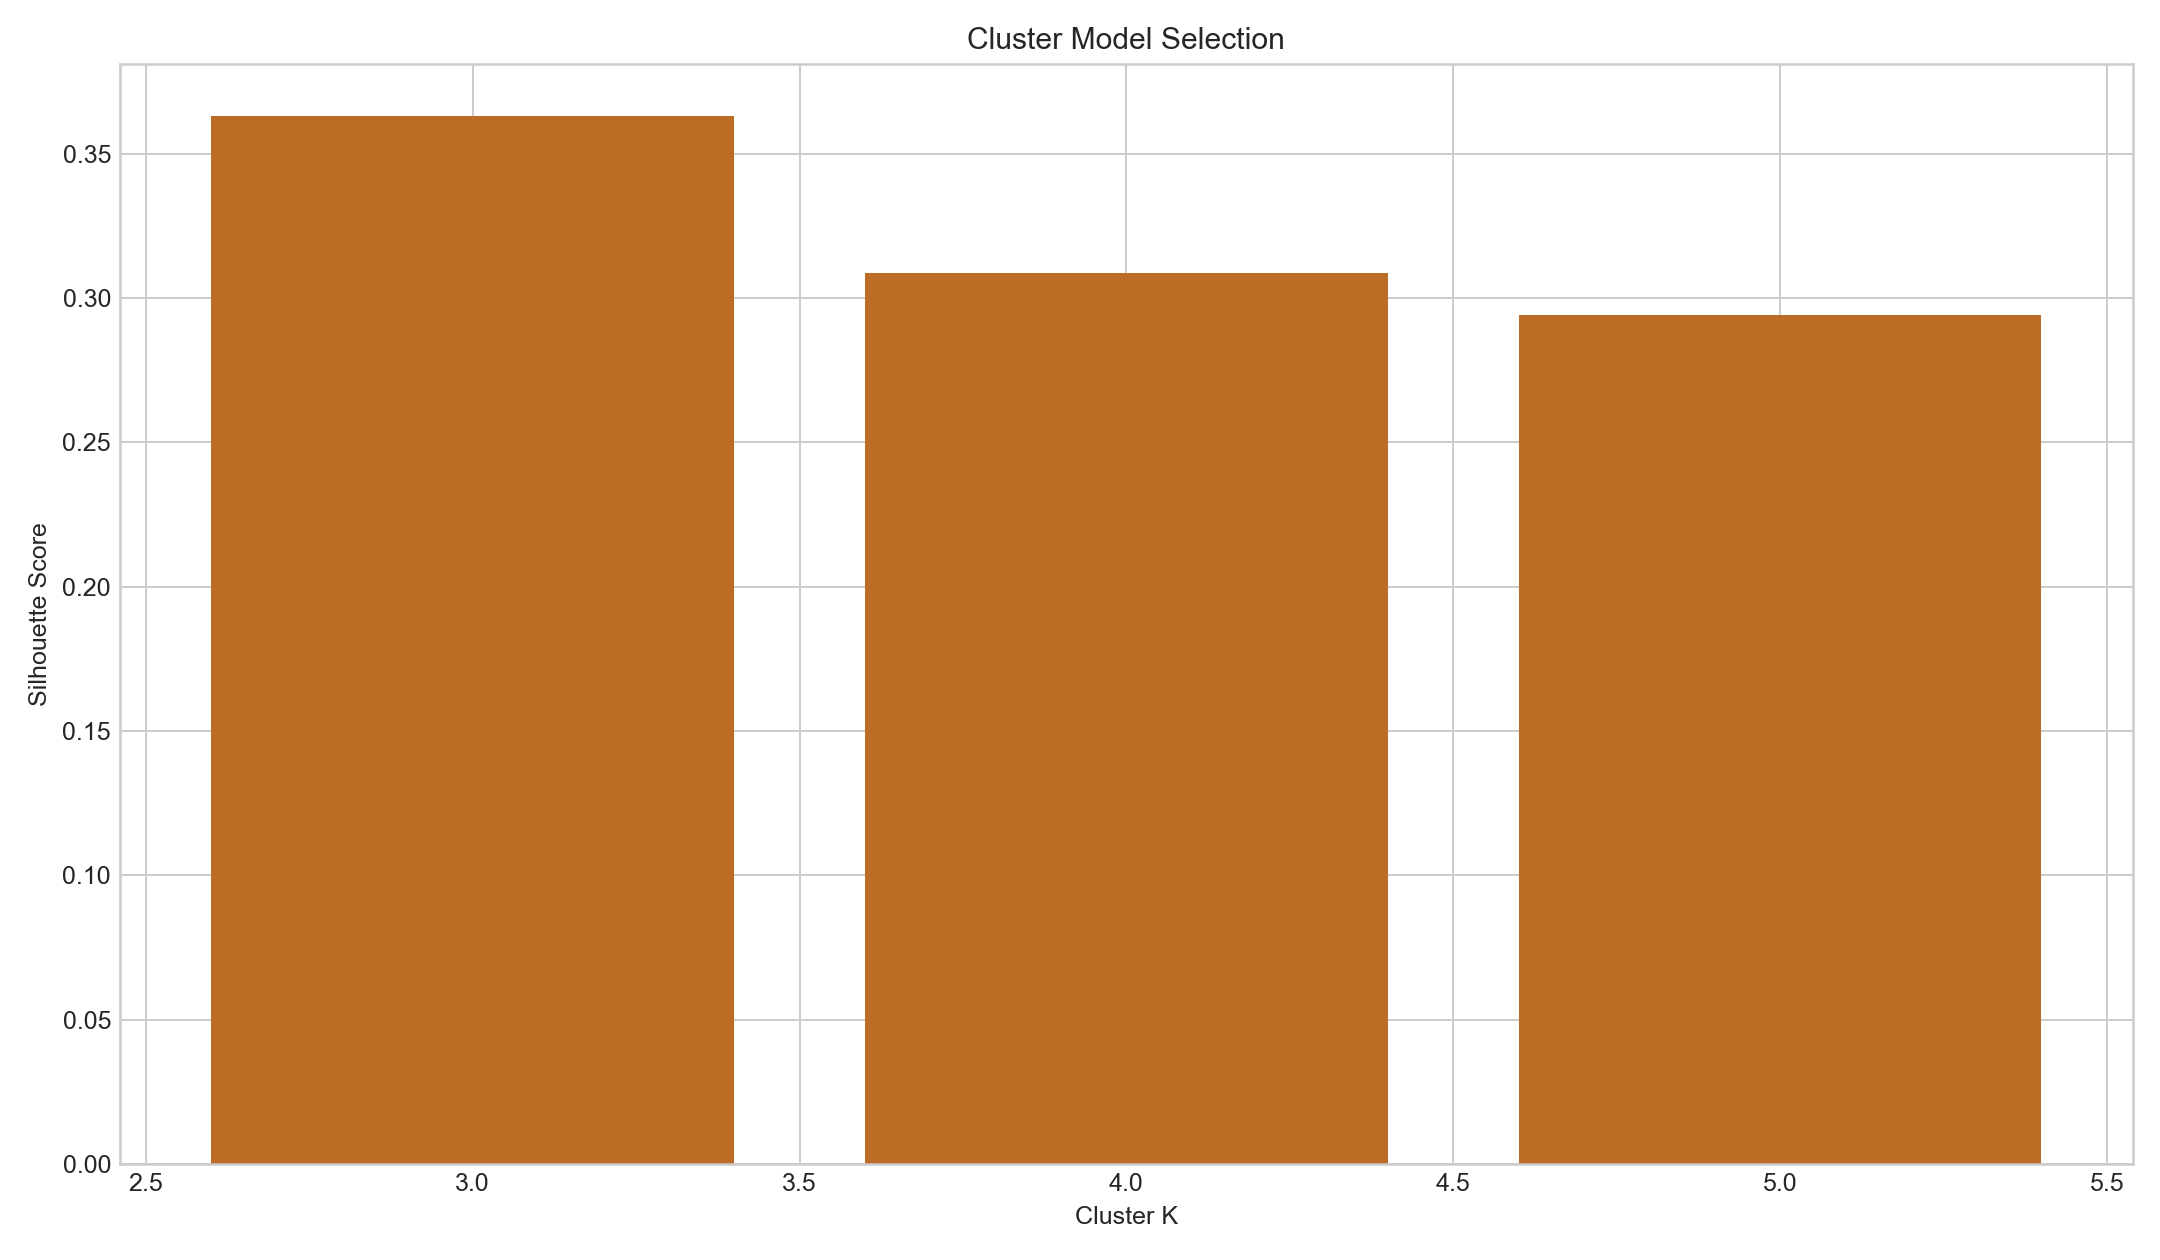
\includegraphics[width=\columnwidth]{13_cluster_k_scores.png}
\caption{Silhouette-score evidence from the persisted \texttt{report\_cluster\_k\_scores} table for tested KMeans configurations.}
\label{fig:k_selection}
\end{figure}

\subsection{Validation, Optimization, and Exploratory Modeling}
The strongest correctness evidence in RetailPulse comes from the validation lane. Table~\ref{tab:stream_validation_expanded} summarizes the persisted \texttt{report\_stream\_validation} outputs at group grain and confirms full agreement with batch recomputation. Table~\ref{tab:olap_validation} complements this result by confirming that base-grain cube totals matched the equivalent direct fact-table aggregation.

The optimization benchmark produced a more nuanced result. As shown in Table~\ref{tab:optimize_summary}, running \texttt{OPTIMIZE} and \texttt{ZORDER BY} on the small sample did not improve the two benchmarked queries. This is not a negative result to hide; it is a reminder that physical optimization should be reported empirically instead of assumed to help.

\textit{Classifier and regression results are exploratory and useful for demo discussion, but not final predictive proof. Methodology tightening is still pending.}

Table~\ref{tab:exploratory_metrics} remains secondary to release-safe validation and recommendation evidence; despite baseline improvements, the current feature-design weaknesses in Section~V prevent production-grade predictive claims.

\begin{table}[!t]
\caption{Expanded replay-stream validation summary derived from persisted \texttt{report\_stream\_validation} output.}
\label{tab:stream_validation_expanded}
\centering
\footnotesize
\begin{tabular}{p{3.6cm} p{2.8cm}}
\toprule
\textbf{Validation field} & \textbf{Value} \\
\midrule
Checked order-slot groups & 158 \\
Mismatched groups & 0 \\
Match rate & 100\% \\
Aggregation grain & (\texttt{order\_dow}, \texttt{order\_hour\_of\_day}) \\
Release criterion & \(M=0\) \\
Release decision & Pass \\
\bottomrule
\end{tabular}
\end{table}

\begin{table}[!t]
\caption{OLAP validation result for the cube cross-check.}
\label{tab:olap_validation}
\centering
\footnotesize
\begin{tabular}{p{4.8cm} p{1.9cm}}
\toprule
\textbf{Check} & \textbf{Result} \\
\midrule
Cube totals compared against direct fact-table aggregation & All matched \\
\bottomrule
\end{tabular}
\end{table}

\begin{table}[!t]
\caption{Benchmark timings before and after optimization.}
\label{tab:optimize_summary}
\centering
\footnotesize
\begin{tabular}{p{2.8cm} r r r}
\toprule
\textbf{Query} & \textbf{Before (s)} & \textbf{After (s)} & \textbf{Delta (s)} \\
\midrule
\texttt{department\_hour\_distribution} & 0.6994 & 0.8350 & +0.1356 \\
\texttt{user\_basket\_summary} & 0.6828 & 0.9789 & +0.2961 \\
\bottomrule
\end{tabular}
\end{table}

\begin{table}[!t]
\caption{Exploratory supervised-model metrics.}
\label{tab:exploratory_metrics}
\centering
\footnotesize
\begin{tabular}{p{4.5cm} r}
\toprule
\textbf{Metric} & \textbf{Value} \\
\midrule
Decision-tree accuracy & 0.9136 \\
Decision-tree AUC & 0.8813 \\
Majority-baseline accuracy & 0.7445 \\
Linear-regression RMSE & 5.0945 \\
Linear-regression \(R^2\) & 0.5580 \\
Mean-baseline RMSE & 7.6627 \\
\bottomrule
\end{tabular}
\end{table}

\section{Limitations and Threats to Validity}
RetailPulse has four main validity limits. First, the source data bounds the problem formulation. Instacart does not contain raw prices, margins, or absolute timestamps, so any claim about revenue, profitability, or calendar seasonality would be unsupported. The framework therefore reports only what the data can honestly sustain.

Second, the platform target constrains implementation choices and performance interpretation. Databricks Free Edition serverless is sufficient for a capstone-scale lakehouse implementation \cite{databricks_free}, but it is not a production environment. That reality shaped the choice of pairwise association rules over more ambitious mining pipelines, the use of \texttt{Trigger.AvailableNow}, and the limited size of the optimization benchmark.

Third, the sampling strategy improves reproducibility at the cost of external validity. The deterministic user-based subsample is suitable for stable reruns and classroom-scale experimentation, but it is still a subset of the original dataset.

Fourth, the supervised-model lane is not yet methodologically rigorous. The clustering notebook includes \texttt{total\_orders} in the feature set, while the classifier predicts a label derived from \texttt{total\_orders} and also consumes \texttt{cluster\_id}. The regression notebook joins user aggregates back into order-level prediction without a strict temporal boundary. These choices make the predictive metrics useful for exploratory discussion, but not for final predictive proof.

\section{Conclusion}
RetailPulse shows that a public grocery dataset, a constrained Databricks environment, and a student-scale engineering scope are still sufficient to produce a credible analytics framework when the pipeline, validation logic, and reporting surfaces are aligned. The system materializes a reproducible bronze--silver--gold Delta workflow, persists OLAP and recommendation evidence, exposes readable customer segments, validates streaming behavior against batch truth, and reports performance outcomes without hiding unfavorable benchmark results.

Future work should extend the framework in three directions: multi-dataset ingestion with explicit dataset identifiers, leakage-safe redesign of the predictive lane, and further dashboard/presentation refinement around the already validated warehouse outputs. Those steps would improve generality and methodological rigor, but the current release already demonstrates the core claim of this paper: RetailPulse is a reproducible, evidence-backed retail analytics framework rather than a disconnected notebook demo.

\bibliographystyle{IEEEtran}
\bibliography{retailpulse_references}

\end{document}
